\documentclass[14pt]{extbook}
\usepackage{multicol, enumerate, enumitem, hyperref, color, soul, setspace, parskip, fancyhdr} %General Packages
\usepackage{amssymb, amsthm, amsmath, bbm, latexsym, units, mathtools} %Math Packages
\everymath{\displaystyle} %All math in Display Style
% Packages with additional options
\usepackage[headsep=0.5cm,headheight=12pt, left=1 in,right= 1 in,top= 1 in,bottom= 1 in]{geometry}
\usepackage[usenames,dvipsnames]{xcolor}
\usepackage{dashrule}  % Package to use the command below to create lines between items
\newcommand{\litem}[1]{\item#1\hspace*{-1cm}\rule{\textwidth}{0.4pt}}
\pagestyle{fancy}
\lhead{Makeup Progress Quiz 3}
\chead{}
\rhead{Version B}
\lfoot{4315-3397}
\cfoot{}
\rfoot{Fall 2020}
\begin{document}

\begin{enumerate}
\litem{
Construct the lowest-degree polynomial given the zeros below. Then, choose the intervals that contain the coefficients of the polynomial in the form $ax^3+bx^2+cx+d$.\[ -1, -6, \text{ and } \frac{5}{2} \]\begin{enumerate}[label=\Alph*.]
\item \( a \in [1, 4], b \in [8, 10.2], c \in [-27, -22], \text{ and } d \in [-36, -26] \)
\item \( a \in [1, 4], b \in [8, 10.2], c \in [-27, -22], \text{ and } d \in [23, 31] \)
\item \( a \in [1, 4], b \in [-19.9, -15.6], c \in [42, 56], \text{ and } d \in [-36, -26] \)
\item \( a \in [1, 4], b \in [-12.1, -5.2], c \in [-27, -22], \text{ and } d \in [23, 31] \)
\item \( a \in [1, 4], b \in [4.5, 8.8], c \in [-39, -32], \text{ and } d \in [23, 31] \)

\end{enumerate} }
\litem{
Construct the lowest-degree polynomial given the zeros below. Then, choose the intervals that contain the coefficients of the polynomial in the form $x^3+bx^2+cx+d$.\[ 4 + 3 i \text{ and } -2 \]\begin{enumerate}[label=\Alph*.]
\item \( b \in [5, 17], c \in [6, 9.1], \text{ and } d \in [-53.4, -49.1] \)
\item \( b \in [0, 4], c \in [-3.7, -1.4], \text{ and } d \in [-11, -7.5] \)
\item \( b \in [-14, 0], c \in [6, 9.1], \text{ and } d \in [49.6, 50.9] \)
\item \( b \in [0, 4], c \in [-1.8, 0.5], \text{ and } d \in [-6.5, -1.6] \)
\item \( \text{None of the above.} \)

\end{enumerate} }
\litem{
Construct the lowest-degree polynomial given the zeros below. Then, choose the intervals that contain the coefficients of the polynomial in the form $x^3+bx^2+cx+d$.\[ -5 + 3 i \text{ and } -1 \]\begin{enumerate}[label=\Alph*.]
\item \( b \in [-9, 7], c \in [-3, 0], \text{ and } d \in [-5, 0] \)
\item \( b \in [-9, 7], c \in [0, 12], \text{ and } d \in [1, 7] \)
\item \( b \in [8, 18], c \in [40, 48], \text{ and } d \in [32, 38] \)
\item \( b \in [-13, -7], c \in [40, 48], \text{ and } d \in [-34, -25] \)
\item \( \text{None of the above.} \)

\end{enumerate} }
\litem{
Construct the lowest-degree polynomial given the zeros below. Then, choose the intervals that contain the coefficients of the polynomial in the form $ax^3+bx^2+cx+d$.\[ 3, \frac{5}{2}, \text{ and } \frac{3}{5} \]\begin{enumerate}[label=\Alph*.]
\item \( a \in [6, 17], b \in [61, 69], c \in [102, 110], \text{ and } d \in [44, 50] \)
\item \( a \in [6, 17], b \in [-3, 3], c \in [-79, -76], \text{ and } d \in [44, 50] \)
\item \( a \in [6, 17], b \in [46, 56], c \in [41, 44], \text{ and } d \in [-48, -41] \)
\item \( a \in [6, 17], b \in [-61, -59], c \in [102, 110], \text{ and } d \in [-48, -41] \)
\item \( a \in [6, 17], b \in [-61, -59], c \in [102, 110], \text{ and } d \in [44, 50] \)

\end{enumerate} }
\litem{
Describe the zero behavior of the zero $x = -5$ of the polynomial below.\[ f(x) = 7(x + 7)^{11}(x - 7)^{8}(x + 5)^{3}(x - 5)^{2} \]\begin{enumerate}[label=\Alph*.]
\begin{multicols}{2}\item 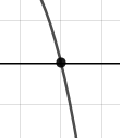
\includegraphics[width = 0.3\textwidth]{../Figures/polyZeroBehaviorAB.png}\item 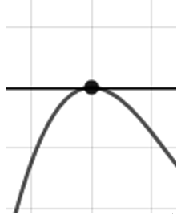
\includegraphics[width = 0.3\textwidth]{../Figures/polyZeroBehaviorBB.png}\item 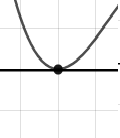
\includegraphics[width = 0.3\textwidth]{../Figures/polyZeroBehaviorCB.png}\item 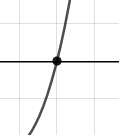
\includegraphics[width = 0.3\textwidth]{../Figures/polyZeroBehaviorDB.png}\end{multicols}\item None of the above.
\end{enumerate} }
\litem{
Which of the following equations \textit{could} be of the graph presented below?
\begin{center}
    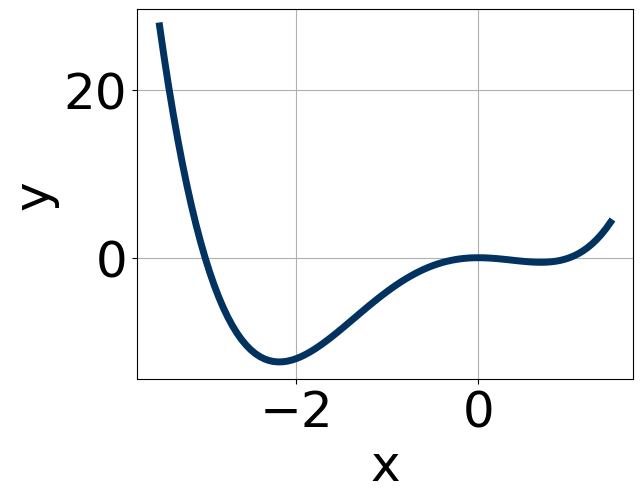
\includegraphics[width=0.5\textwidth]{../Figures/polyGraphToFunctionCopyB.png}
\end{center}
\begin{enumerate}[label=\Alph*.]
\item \( 4x^{8} (x - 1)^{6} (x + 3)^{9} \)
\item \( 7x^{6} (x - 1)^{5} (x + 3)^{9} \)
\item \( -19x^{8} (x - 1)^{7} (x + 3)^{7} \)
\item \( -10x^{10} (x - 1)^{11} (x + 3)^{10} \)
\item \( 9x^{11} (x - 1)^{10} (x + 3)^{9} \)

\end{enumerate} }
\litem{
Describe the zero behavior of the zero $x = -3$ of the polynomial below.\[ f(x) = 9(x + 3)^{3}(x - 3)^{8}(x + 2)^{4}(x - 2)^{5} \]\begin{enumerate}[label=\Alph*.]
\begin{multicols}{2}\item 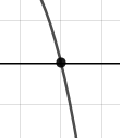
\includegraphics[width = 0.3\textwidth]{../Figures/polyZeroBehaviorCopyAB.png}\item 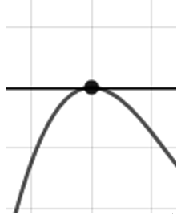
\includegraphics[width = 0.3\textwidth]{../Figures/polyZeroBehaviorCopyBB.png}\item 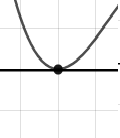
\includegraphics[width = 0.3\textwidth]{../Figures/polyZeroBehaviorCopyCB.png}\item 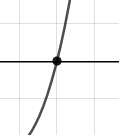
\includegraphics[width = 0.3\textwidth]{../Figures/polyZeroBehaviorCopyDB.png}\end{multicols}\item None of the above.
\end{enumerate} }
\litem{
Which of the following equations \textit{could} be of the graph presented below?
\begin{center}
    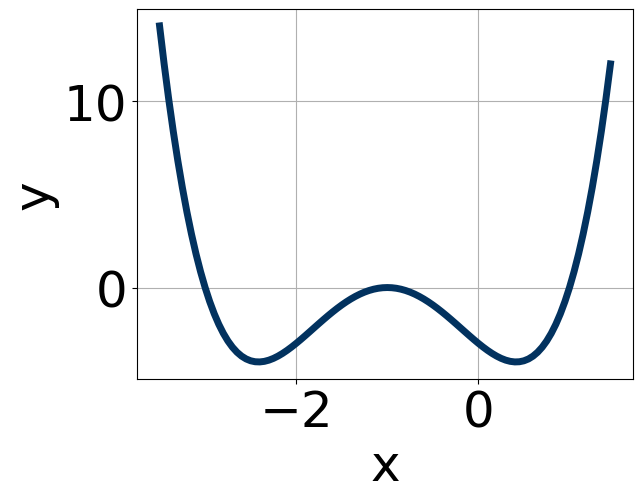
\includegraphics[width=0.5\textwidth]{../Figures/polyGraphToFunctionB.png}
\end{center}
\begin{enumerate}[label=\Alph*.]
\item \( 17(x + 1)^{8} (x + 3)^{11} (x - 1)^{11} \)
\item \( -18(x + 1)^{10} (x + 3)^{5} (x - 1)^{8} \)
\item \( 11(x + 1)^{8} (x + 3)^{8} (x - 1)^{11} \)
\item \( -10(x + 1)^{6} (x + 3)^{11} (x - 1)^{9} \)
\item \( 11(x + 1)^{5} (x + 3)^{6} (x - 1)^{9} \)

\end{enumerate} }
\litem{
Describe the end behavior of the polynomial below.\[ f(x) = 7(x + 6)^{4}(x - 6)^{5}(x - 8)^{5}(x + 8)^{5} \]\begin{enumerate}[label=\Alph*.]
\begin{multicols}{2}\item 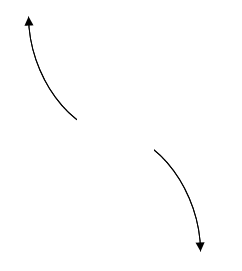
\includegraphics[width = 0.3\textwidth]{../Figures/polyEndBehaviorCopyAB.png}\item 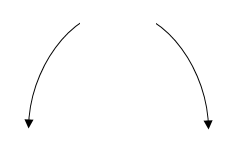
\includegraphics[width = 0.3\textwidth]{../Figures/polyEndBehaviorCopyBB.png}\item 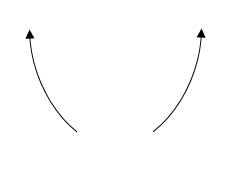
\includegraphics[width = 0.3\textwidth]{../Figures/polyEndBehaviorCopyCB.png}\item 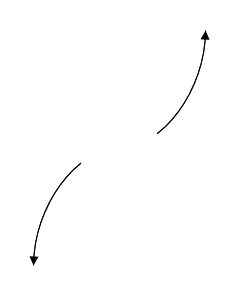
\includegraphics[width = 0.3\textwidth]{../Figures/polyEndBehaviorCopyDB.png}\end{multicols}\item None of the above.
\end{enumerate} }
\litem{
Describe the end behavior of the polynomial below.\[ f(x) = -5(x + 7)^{2}(x - 7)^{3}(x + 3)^{2}(x - 3)^{4} \]\begin{enumerate}[label=\Alph*.]
\begin{multicols}{2}\item 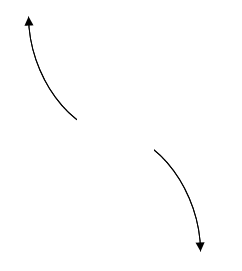
\includegraphics[width = 0.3\textwidth]{../Figures/polyEndBehaviorAB.png}\item 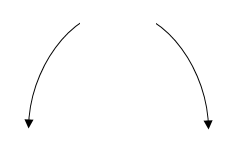
\includegraphics[width = 0.3\textwidth]{../Figures/polyEndBehaviorBB.png}\item 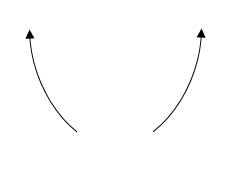
\includegraphics[width = 0.3\textwidth]{../Figures/polyEndBehaviorCB.png}\item 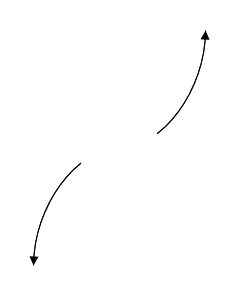
\includegraphics[width = 0.3\textwidth]{../Figures/polyEndBehaviorDB.png}\end{multicols}\item None of the above.
\end{enumerate} }
\end{enumerate}

\end{document}